% STRUCTURAL MASONRY
Structural masonry is a composite material that consists of brick units and mortar.
A simplified sketch is found in \cref{fig:ICASP:Masonry}.
% COMPRESSIVE STRENGTH
The mechanical key characteristic of masonry is the compressive strength perpendicular to the bed joints.
Estimating or predicting this material property are thus issues of central importance to assessing the reliability of masonry structures.
% CURRENT MODELS
These problems are therefore addressed in current standards \cite{Standard:Eurocode6:1-1,Standard:JCSSProbabilisticCode} and numerous enhancements
\cite{Masonry:Dymiotis2002,Masonry:Glowienka2006,Masonry:Schueremans2006,Masonry:Mojsilovic2009,Masonry:Sykora2010,Masonry:GarzonRoca2013,Masonry:Sykora2014:a,Masonry:Sykora2014:b}.
% STRUCTURAL MASONRY
\begin{figure}[tb]
  \centering
  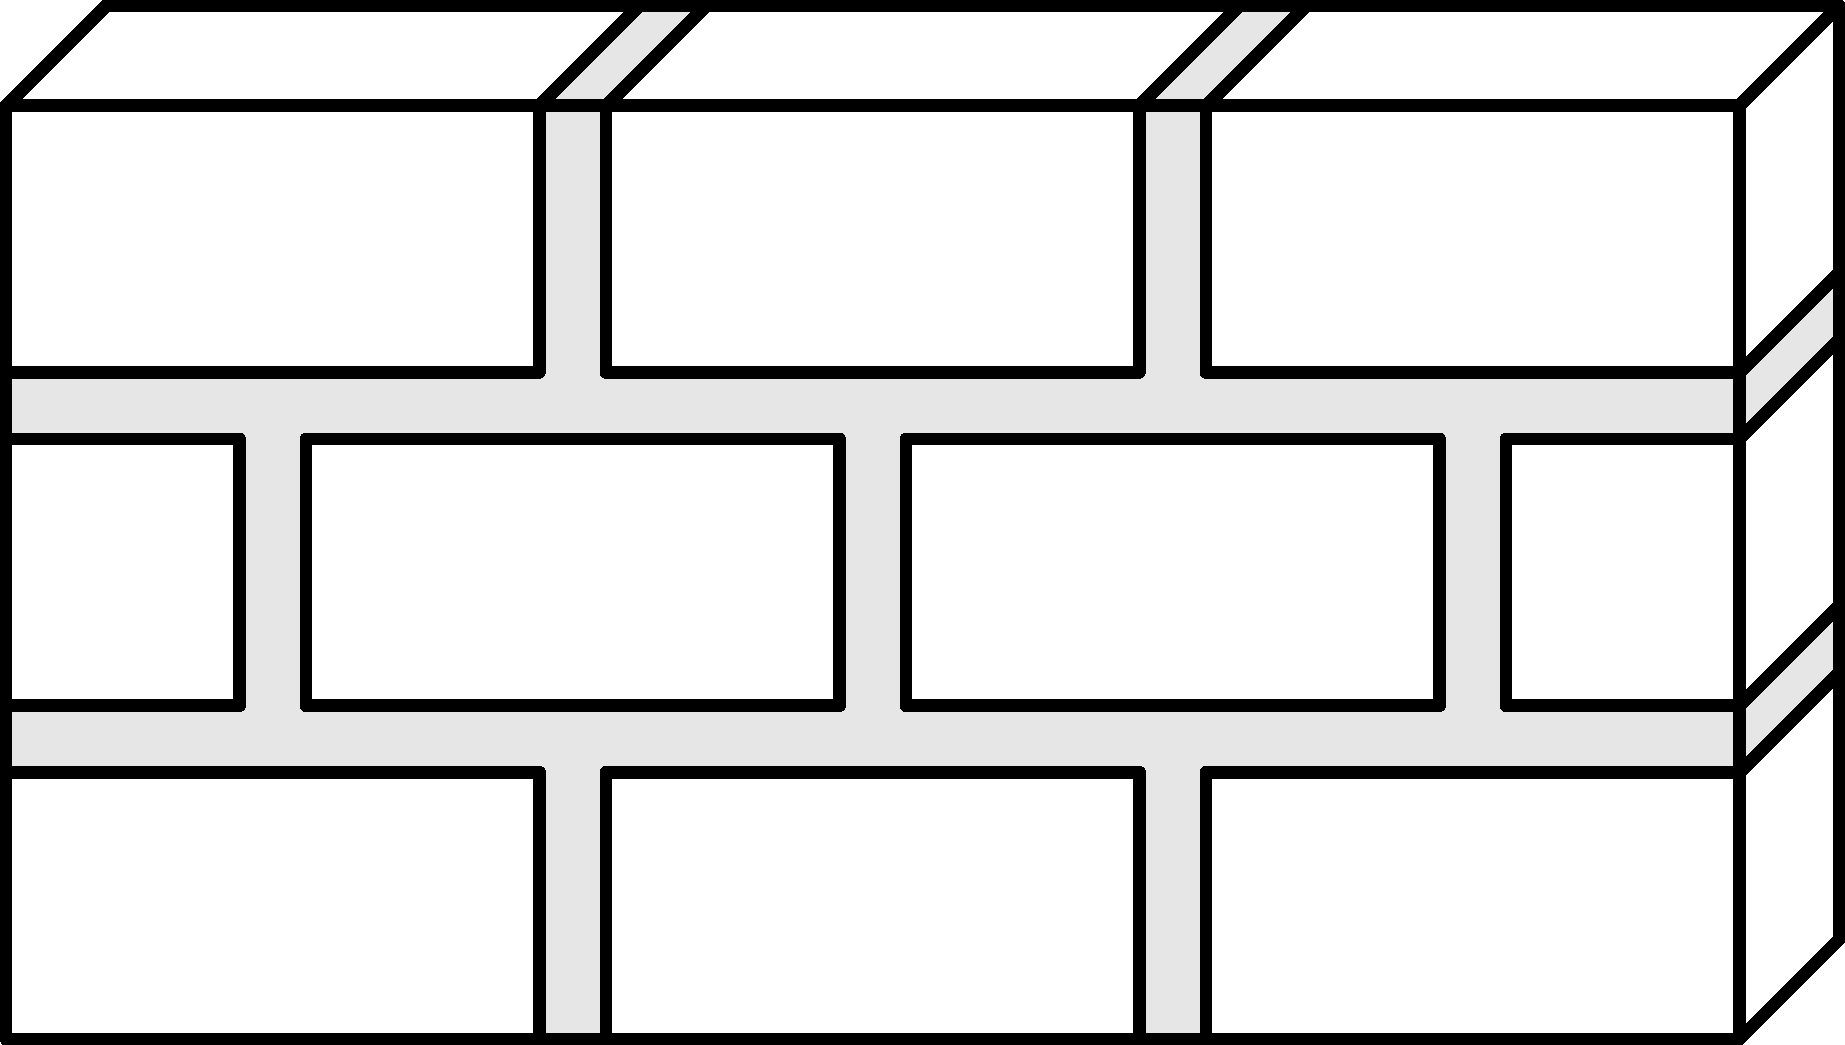
\includegraphics[width=5cm]{fig_ICASP_Masonry}
  \caption[Structural masonry]{Structural masonry.
           The masonry wall is composed of brick units (white) that are bound by mortar (gray).
          }
  \label{fig:ICASP:Masonry}
\end{figure}
\par % MOTIVATION
The motivation of this research study is twofold.
Firstly, we observe a systematic discrepancy between measured data and predictions of the masonry compressive strength according to \cite{Standard:Eurocode6:1-1}.
This suggests a recalibration of the model code parameters.
Secondly, it is noticed that current approaches either suffer from their semi-probabilistic character or their unsatisfactory treatment of the emerging uncertainties.
% GENERAL GOAL
Thus the goal of this paper is to develop a fully probabilistic extension of current codified models for assessing the compressive strength of unreinforced masonry.
% METHODOLOGY
We will rely on hierarchical models \cite{Nagel:JAIS2015,Nagel:PEM2016} and Bayesian networks \cite{Multilevel:Sankararaman2012,Bayesian:Urbina2012}.
This approach will allow for heterogeneous modeling of structural masonry, quantification of various types of uncertainty and acquisition of information from diverse sources.
\par % EXPERIMENTAL SCENARIO
More specifically it is aimed at analyzing the compressive strength of structural masonry with system-level data, i.e.\ measurements that are taken from full-scale masonry specimens,  
component-level data, i.e.\ results from testing brick units and mortar samples individually, and prior or expert knowledge.
Compression tests of masonry specimens are rather costly, whereas data associated to component-specific material characteristics are relatively inexpensive to acquire.
Hierarchical models enable the joint processing of information from different levels of the overall system.
This way the information is optimally utilized.
Moreover a predictive relationship is established that connects the masonry compressive strength with the component-level compressive strengths.
\par % OUTLINE
The remainder of this document is organized as follows.
Previous approaches of assessing the compressive strength of structural masonry will be reviewed in \cref{sec:ICASP:Previous}.
Hierarchical models will be introduced in \cref{sec:ICASP:Networks}.
In \cref{sec:ICASP:Data} the acquired data will be discussed and \cref{sec:ICASP:Analysis} will show the results of Bayesian updating.
Lastly we will summarize and conclude in \cref{sec:ICASP:Conclusion}.